% LaTeX-Vorlage für Versuchsprotokolle
% Autor: Simon May
% Datum: 2017-10-05

% Es gibt die Dokumenttypen scrartcl („Artikel“), scrreprt („Bericht“),
% scrbook („Buch“) und scrlttr2 („Brief“). Diese gehören zum KOMA-Script,
% bieten mehr Optionen als die „Standardklassen“ und sollten besonders für
% deutsche Texte benutzt werden.
% Natürlich gibt es noch weitere Klassen, z.B. beamer für Präsentationen.
\documentclass[
	a4paper,                % Papierformat (DIN A4)
	titlepage=firstiscover, % Separate Titelseite
	captions=tableheading,  % \caption bei Tabellen immer als Überschrift setzen
	toc=bibliography,       % Literaturverzeichnis im Inhaltsverzeichnis aufführen
	toc=listof,             % Abbildungsverzeichnis etc. im Inhaltsverzeichnis aufführen
	oneside,                % Einseitig
	%twoside,               % Zweiseitig
	%twocolumn,             % Zweispaltig
	automark,               % Abschnittstitel automatisch in Kopfzeile einfügen
	12pt,                   % Schriftgröße (beliebige Größen mit „fontsize=Xpt“)
	english, ngerman,       % Sprache für z.B. Babel; ausgewählt: ngerman (letztgenannt)
	%draft=true             % Entwurf-Modus; markiert zu lange und zu kurze Zeilen
]{scrartcl}

% --- Pakete einbinden
% Autor: Simon May
% Datum: 2017-10-04

% --- Pakete einbinden
% --- Pakete erweitern LaTeX um zusätzliche Funktionen.
%     Dies ist ein Satz nützlicher Pakete.

% Silbentrennung etc.; Sprache wird durch Option bei \documentclass festgelegt
\usepackage{babel}
\usepackage{iftex}
\ifLuaTeX
	% Schriftart (Latin Modern)
	\usepackage{fontspec}
	\fontspec{Latin Modern Roman}
\else
	% Verwendung der Zeichentabelle T1 (für Sonderzeichen etc.)
	\usepackage[T1]{fontenc}
	% Legt die Eingabe-Zeichenkodierung fest, z.B. UTF-8
	\usepackage[utf8]{inputenc}
	% Schriftart (Latin Modern)
	\usepackage{lmodern}
	% Zusätzliche Sonderzeichen
	\usepackage{textcomp}
\fi

% Nutzen von +, -, *, / in \setlength u.ä. (z.B. \setlength{\a + 3cm})
\usepackage{calc}
% Wird benötigt, um \ifthenelse zu benutzen
\usepackage{xifthen}
% Optionen für eigene definierte Befehle
\usepackage{xparse}

% Verbessertes Aussehen des Schriftbilds durch kleine Anpassungen
\usepackage{microtype}
% Automatische Formatierung von Daten
\usepackage[useregional]{datetime2}
% Wird für Kopf- und Fußzeile benötigt
\usepackage{scrlayer-scrpage}
% Einfaches Wechseln zwischen unterschiedlichen Zeilenabständen
\usepackage{setspace}
% Optionen für Listen (enumerate, itemize, …)
\usepackage{enumitem}
% Automatische Anführungszeichen
\usepackage{csquotes}
% Zusätzliche Optionen für Tabellen (tabular)
\usepackage{array}

% Mathepaket (intlimits: Grenzen über/unter Integralzeichen)
\usepackage[intlimits]{amsmath}
% Mathe-Symbole, \mathbb etc.
\usepackage{amssymb}
% Weitere Mathebefehle
\usepackage{mathtools}
% „Schöne“ Brüche im Fließtext
\usepackage{xfrac}
% Ermöglicht die Nutzung von \SI{Zahl}{Einheit} u.a.
\usepackage{siunitx}
% Definition von Unicode-Symbolen; Nach [utf8]inputenc laden!
\usepackage{newunicodechar}
% Unicode-Formeln mit pdfLaTeX
% Autor: Simon May
% Datum: 2015-03-04

% Diese Datei ermöglicht es, Mathe-Symbole (z.B. \gamma) direkt als
% Sonderzeichen (d.h. γ) einzugeben

% silence unterdrückt Warnungen; vor hyperref laden
\usepackage{silence}
\WarningFilter[pdflatex-unicode-math]{newunicodechar}{Redefining Unicode character}
\ActivateWarningFilters[pdflatex-unicode-math]

\newunicodechar{†}{\dag}
\newunicodechar{‡}{\ddag}
\newunicodechar{…}{\ldots}
\newunicodechar{⋯}{\cdots}
\newunicodechar{⋮}{\vdots}
\newunicodechar{⋱}{\ddots}
\newunicodechar{⋰}{\iddots}
\newunicodechar{α}{\alpha}
\newunicodechar{β}{\beta}
\newunicodechar{γ}{\gamma}
\newunicodechar{δ}{\delta}
\newunicodechar{ε}{\varepsilon}
\newunicodechar{ϵ}{\epsilon}
\newunicodechar{ζ}{\zeta}
\newunicodechar{η}{\eta}
\newunicodechar{θ}{\theta}
\newunicodechar{ϑ}{\vartheta}
\newunicodechar{ι}{\iota}
\newunicodechar{κ}{\kappa}
\newunicodechar{ϰ}{\varkappa}
\newunicodechar{λ}{\lambda}
\newunicodechar{μ}{\mu}
\newunicodechar{ν}{\nu}
\newunicodechar{ξ}{\xi}
\newunicodechar{ο}{o}
\newunicodechar{π}{\pi}
\newunicodechar{ρ}{\rho}
\newunicodechar{ϱ}{\varrho}
\newunicodechar{σ}{\sigma}
\newunicodechar{τ}{\tau}
\newunicodechar{υ}{\upsilon}
\newunicodechar{φ}{\varphi}
\newunicodechar{ϕ}{\phi}
\newunicodechar{χ}{\chi}
\newunicodechar{ψ}{\psi}
\newunicodechar{ω}{\omega}
\newunicodechar{Α}{\mathrm{A}}
\newunicodechar{Β}{\mathrm{B}}
\newunicodechar{Γ}{\Gamma}
\newunicodechar{Δ}{\Delta}
\newunicodechar{Ε}{\mathrm{E}}
\newunicodechar{Ζ}{\mathrm{Z}}
\newunicodechar{Η}{\mathrm{H}}
\newunicodechar{Θ}{\Theta}
\newunicodechar{Ι}{\mathrm{I}}
\newunicodechar{Κ}{\mathrm{K}}
\newunicodechar{Λ}{\Lambda}
\newunicodechar{Μ}{\mathrm{M}}
\newunicodechar{Ν}{\mathrm{N}}
\newunicodechar{Ξ}{\Xi}
\newunicodechar{Ο}{\mathrm{O}}
\newunicodechar{Π}{\Pi}
\newunicodechar{Ρ}{\mathrm{P}}
\newunicodechar{Σ}{\Sigma}
\newunicodechar{Τ}{\mathrm{T}}
\newunicodechar{Υ}{\Upsilon}
\newunicodechar{Φ}{\Phi}
\newunicodechar{Χ}{\Chi}
\newunicodechar{Ψ}{\Psi}
\newunicodechar{Ω}{\Omega}
\newunicodechar{∑}{\sum}
\newunicodechar{∫}{\int}
\newunicodechar{∬}{\iint}
\newunicodechar{∭}{\iiint}
\newunicodechar{⨌}{\iiiint}
\newunicodechar{∮}{\oint}
\newunicodechar{∯}{\oiint}
\newunicodechar{∰}{\oiiint}
\newunicodechar{∇}{\nabla}
\newunicodechar{∂}{\partial}
\newunicodechar{√}{\sqrt}
\newunicodechar{∈}{\in}
\newunicodechar{∋}{\ni}
\newunicodechar{∉}{\notin}
\newunicodechar{∀}{\forall}
\newunicodechar{∃}{\exists}
\newunicodechar{∄}{\nexists}
\newunicodechar{∴}{\therefore}
\newunicodechar{∵}{\because}
\newunicodechar{〈}{\langle}
\newunicodechar{〉}{\rangle}
\newunicodechar{⌊}{\lfloor}
\newunicodechar{⌋}{\rfloor}
\newunicodechar{⌈}{\lceil}
\newunicodechar{⌉}{\rceil}
\newunicodechar{∼}{\sim}
\newunicodechar{∝}{\propto}
\newunicodechar{∞}{\infty}
\newunicodechar{ℵ}{\aleph}
\newunicodechar{ℏ}{\hbar}
\newunicodechar{℘}{\wp}
\newunicodechar{ℓ}{\ell}
\newunicodechar{∅}{\emptyset}
\newunicodechar{×}{\times}
\newunicodechar{⋅}{\cdot}
\newunicodechar{÷}{\div}
\newunicodechar{⋆}{\star}
\newunicodechar{∘}{\circ}
\newunicodechar{⋄}{\diamond}
\newunicodechar{⊕}{\oplus}
\newunicodechar{⊖}{\ominus}
\newunicodechar{⊗}{\otimes}
\newunicodechar{⊘}{\oslash}
\newunicodechar{⊙}{\odot}
\newunicodechar{±}{\pm}
\newunicodechar{∓}{\mp}
\newunicodechar{≈}{\approx}
\newunicodechar{≡}{\equiv}
\newunicodechar{≠}{\ne}
\newunicodechar{≥}{\ge}
\newunicodechar{≤}{\le}
\newunicodechar{≫}{\gg}
\newunicodechar{≪}{\ll}
\newunicodechar{⊂}{\subset}
\newunicodechar{⊃}{\supset}
\newunicodechar{⊆}{\subseteq}
\newunicodechar{⊇}{\supseteq}
\newunicodechar{⊈}{\nsubseteq}
\newunicodechar{⊉}{\nsupseteq}
\newunicodechar{≔}{\coloneqq}
\newunicodechar{≕}{\eqqcolon}
\newunicodechar{¬}{\neg}
\newunicodechar{∨}{\vee}
\newunicodechar{∧}{\wedge}
\newunicodechar{∪}{\cup}
\newunicodechar{∩}{\cap}
\newunicodechar{⋁}{\bigvee}
\newunicodechar{⋀}{\bigwedge}
\newunicodechar{⋃}{\bigcup}
\newunicodechar{⋂}{\bigcap}
\newunicodechar{⟂}{\perp}
\newunicodechar{∥}{\parallel}
\newunicodechar{∦}{\nparallel}
\newunicodechar{𝚤}{\imath}
\newunicodechar{𝚥}{\jmath}
\newunicodechar{⇔}{\Leftrightarrow}
\newunicodechar{⇕}{\Updownarrow}
\newunicodechar{⇐}{\Leftarrow}
\newunicodechar{⇒}{\Rightarrow}
\newunicodechar{⇑}{\Uparrow}
\newunicodechar{⇓}{\Downarrow}
\newunicodechar{↔}{\leftrightarrow}
\newunicodechar{↕}{\updownarrow}
\newunicodechar{←}{\leftarrow}
\newunicodechar{→}{\rightarrow}
\newunicodechar{↑}{\uparrow}
\newunicodechar{↓}{\downarrow}
\newunicodechar{⟷}{\longleftrightarrow}
\newunicodechar{⟵}{\longleftarrow}
\newunicodechar{⟶}{\longrightarrow}
\newunicodechar{⇇}{\leftleftarrows}
\newunicodechar{⇉}{\rightrightarrows}
\newunicodechar{⇈}{\upuparrows}
\newunicodechar{⇊}{\downdownarrows}
\newunicodechar{⟺}{\Longleftrightarrow}
\newunicodechar{⟸}{\Longleftarrow}
\newunicodechar{⟹}{\Longrightarrow}
\newunicodechar{↦}{\mapsto}
\newunicodechar{↤}{\mapsfrom}
\newunicodechar{⟼}{\longmapsto}
\newunicodechar{⟻}{\longmapsfrom}
\newunicodechar{⟾}{\Longmapsto}
\newunicodechar{⟽}{\Longmapsfrom}
\newunicodechar{↗}{\nearrow}
\newunicodechar{↖}{\nwarrow}
\newunicodechar{↘}{\searrow}
\newunicodechar{↙}{\swarrow}
\newunicodechar{↩}{\hookleftarrow}
\newunicodechar{↪}{\hookrightarrow}
\newunicodechar{↶}{\curvearrowleft}
\newunicodechar{↷}{\curvearrowright}
\newunicodechar{↺}{\circlearrowleft}
\newunicodechar{↻}{\circlearrowright}
\newunicodechar{↫}{\looparrowleft}
\newunicodechar{↬}{\looparrowright}
\newunicodechar{⇋}{\leftrightharpoons}
\newunicodechar{⇌}{\rightleftharpoons}
\newunicodechar{↼}{\leftharpoonup}
\newunicodechar{↽}{\leftharpoondown}
\newunicodechar{⇀}{\rightharpoonup}
\newunicodechar{⇁}{\rightharpoondown}
\newunicodechar{↿}{\upharpoonleft}
\newunicodechar{↾}{\upharpoonright}
\newunicodechar{⇃}{\downharpoonleft}
\newunicodechar{⇂}{\downharpoonright}
\newunicodechar{𝔸}{\mathbb{A}}
\newunicodechar{𝔹}{\mathbb{B}}
\newunicodechar{ℂ}{\mathbb{C}}
\newunicodechar{𝔻}{\mathbb{D}}
\newunicodechar{𝔼}{\mathbb{E}}
\newunicodechar{𝔽}{\mathbb{F}}
\newunicodechar{𝔾}{\mathbb{G}}
\newunicodechar{ℍ}{\mathbb{H}}
\newunicodechar{𝕀}{\mathbb{I}}
\newunicodechar{𝕁}{\mathbb{J}}
\newunicodechar{𝕂}{\mathbb{K}}
\newunicodechar{𝕃}{\mathbb{L}}
\newunicodechar{𝕄}{\mathbb{M}}
\newunicodechar{ℕ}{\mathbb{N}}
\newunicodechar{𝕆}{\mathbb{O}}
\newunicodechar{ℙ}{\mathbb{P}}
\newunicodechar{ℚ}{\mathbb{Q}}
\newunicodechar{ℝ}{\mathbb{R}}
\newunicodechar{𝕊}{\mathbb{S}}
\newunicodechar{𝕋}{\mathbb{T}}
\newunicodechar{𝕌}{\mathbb{U}}
\newunicodechar{𝕍}{\mathbb{V}}
\newunicodechar{𝕎}{\mathbb{W}}
\newunicodechar{𝕏}{\mathbb{X}}
\newunicodechar{𝕐}{\mathbb{Y}}
\newunicodechar{ℤ}{\mathbb{Z}}
\newunicodechar{𝒜}{\mathcal{A}}
\newunicodechar{ℬ}{\mathcal{B}}
\newunicodechar{𝒞}{\mathcal{C}}
\newunicodechar{𝒟}{\mathcal{D}}
\newunicodechar{ℰ}{\mathcal{E}}
\newunicodechar{ℱ}{\mathcal{F}}
\newunicodechar{𝒢}{\mathcal{G}}
\newunicodechar{ℋ}{\mathcal{H}}
\newunicodechar{ℐ}{\mathcal{I}}
\newunicodechar{𝒥}{\mathcal{J}}
\newunicodechar{𝒦}{\mathcal{K}}
\newunicodechar{ℒ}{\mathcal{L}}
\newunicodechar{ℳ}{\mathcal{M}}
\newunicodechar{𝒩}{\mathcal{N}}
\newunicodechar{𝒪}{\mathcal{O}}
\newunicodechar{𝒫}{\mathcal{P}}
\newunicodechar{𝒬}{\mathcal{Q}}
\newunicodechar{ℛ}{\mathcal{R}}
\newunicodechar{𝒮}{\mathcal{S}}
\newunicodechar{𝒯}{\mathcal{T}}
\newunicodechar{𝒰}{\mathcal{U}}
\newunicodechar{𝒱}{\mathcal{V}}
\newunicodechar{𝒲}{\mathcal{W}}
\newunicodechar{𝒳}{\mathcal{X}}
\newunicodechar{𝒴}{\mathcal{Y}}
\newunicodechar{𝒵}{\mathcal{Z}}
\newunicodechar{𝕬}{\mathfrak{A}}
\newunicodechar{𝕭}{\mathfrak{B}}
\newunicodechar{𝕮}{\mathfrak{C}}
\newunicodechar{𝕯}{\mathfrak{D}}
\newunicodechar{𝕰}{\mathfrak{E}}
\newunicodechar{𝕱}{\mathfrak{F}}
\newunicodechar{𝕲}{\mathfrak{G}}
\newunicodechar{𝕳}{\mathfrak{H}}
\newunicodechar{𝕴}{\mathfrak{I}}
\newunicodechar{𝕵}{\mathfrak{J}}
\newunicodechar{𝕶}{\mathfrak{K}}
\newunicodechar{𝕷}{\mathfrak{L}}
\newunicodechar{𝕸}{\mathfrak{M}}
\newunicodechar{𝕹}{\mathfrak{N}}
\newunicodechar{𝕺}{\mathfrak{O}}
\newunicodechar{𝕻}{\mathfrak{P}}
\newunicodechar{𝕼}{\mathfrak{Q}}
\newunicodechar{𝕽}{\mathfrak{R}}
\newunicodechar{𝕾}{\mathfrak{S}}
\newunicodechar{𝕿}{\mathfrak{T}}
\newunicodechar{𝖀}{\mathfrak{U}}
\newunicodechar{𝖁}{\mathfrak{V}}
\newunicodechar{𝖂}{\mathfrak{W}}
\newunicodechar{𝖃}{\mathfrak{X}}
\newunicodechar{𝖄}{\mathfrak{Y}}
\newunicodechar{𝖅}{\mathfrak{Z}}

\DeactivateWarningFilters[pdflatex-unicode-math]


% Farben
\usepackage{xcolor}
% Einbinden von Grafiken (\includegraphics)
\usepackage{graphicx}
% .tex-Dateien mit \includegraphics einbinden
\usepackage{gincltex}
% Größere Freiheiten bei Dateinamen mit \includegraphics
\usepackage{grffile}
% Abbildungen im Fließtext
\usepackage{wrapfig}
% Zitieren, Bibliographie (Biber als Bibliographie-Programm verwenden!)
\usepackage[style=verbose, backend=biber]{biblatex}
% Abbildungen nebeneinander (subfigure, subtable)
\usepackage{subcaption}

% Verlinkt Textstellen im PDF-Dokument (sollte am Ende geladen werden)
\usepackage[unicode]{hyperref}
% „Schlaue“ Referenzen (nach hyperref laden!)
\usepackage{cleveref}
%PDF einbinden
%\usepackage{pdfpages}
%Graphiken zeichnen
%\usepackage{tikz}
%\usetikzlibrary{angles,quotes,babel,3d}
% --- Einstellungen
% -- LaTeX/KOMA
% 1,5-facher Zeilenabstand
\onehalfspacing
\recalctypearea
% Schrift bei Bildunterschriften ändern
\addtokomafont{caption}{\small}
\addtokomafont{captionlabel}{\bfseries}
% Nummerierung der Formeln entsprechend des Abschnitts (z.B. 1.1)
\numberwithin{equation}{section}
% „Verwaiste“ Zeilen am Seitenanfang/-Ende stärker vermeiden
\clubpenalty=1000
\widowpenalty=1000
% Auf mehrere Seiten aufgespaltene Fußnoten stärker vermeiden
\interfootnotelinepenalty=3000

% -- csquotes
% Anführungszeichen automatisch umwandeln
\MakeOuterQuote{"}

% -- siunitx
\sisetup{
	locale=DE,
	separate-uncertainty,
	output-product=\cdot,
	quotient-mode=fraction,
	per-mode=fraction,
	fraction-function=\sfrac
}

% -- hyperref
\hypersetup{
	% Links/Verweise mit Kasten der Dicke 0.5pt versehen
	pdfborder={0 0 0.5}
}

% -- cleveref
\crefname{equation}{}{}
\Crefname{equation}{}{}

% -- biblatex (Literaturverzeichnis)
\IfFileExists{res/literatur.bib}{
	\addbibresource{res/literatur.bib}
}{}

\AtEndPreamble{
	% Kopf- und Fußzeile konfigurieren
	\ifthenelse{\boolean{showHeader}}{
		\KOMAoptions{headsepline}
		\recalctypearea
		\automark{section}
		% Innenseite der Kopfzeile
		\ihead{\headmark}
		% Mitte der Kopfzeile
		\chead{}
		% Außenseite der Kopfzeile
		\ohead{\usekomafont{pagehead}\varAutor}
	}{}
	% Innnenseite der Fußzeile
	\ifoot{}
	% Mitte der Fußzeile          
	\cfoot{-~\pagemark~-}
	% Außenseite der Fußzeile
	\ofoot{}

	% Metadaten für die PDF-Datei
	\hypersetup{
		pdftitle={Versuchsprotokoll: \varName},
		pdfauthor={\varAutor},
		pdfsubject={Grundpraktikum},
		pdfkeywords={Physik, Münster, Praktikum, Versuchsprotokoll}
	}
}



% --- Eigene Befehle einbinden
% Autor: Simon May
% Datum: 2017-10-05

% Eigene Befehle eignen sich gut, um Abkürzungen für lange Befehle zu erstellen.
% So vermeidet man, dass man immer wieder dasselbe Konstrukt kopieren und
% einfügen muss und, wenn man dann doch etwas ändern will, an zahllosen Stellen
% im Dokument dieselbe Änderung vornehmen muss.
% Die Syntax ist die folgende:
% \newcommand{neuer Befahl}[Anzahl Parameter (optional)]{Inhalt}
% Das folgende Beispiel fügt ein Bild mit bestimmten vorgegebenen Optionen ein:
\newcommand{\centeredImage}[1]{
	\begin{figure}
		\centering
		\includegraphics[width=0.5\textwidth]{#1}
	\end{figure}
}
% #1 ist dabei ein Parameter, den man \centeredImage übergeben muss, also:
% \centeredImage{...}
% Benötigt man keine Parameter, dann lässt man [1] weg. Werden zusätzliche
% Parameter benötigt, dann kann man die Zahl auf maximal 9 erhöhen.

% Ein Befehl, um eine E-Mail-Adresse darzustellen bzw. automatisch zu verlinken
\newcommand{\email}[1]{\href{mailto:#1}{\texttt{#1}}}

% \arsinh etc.
\newcommand*{\arsinh}{\operatorname{arsinh}}
\newcommand*{\arcosh}{\operatorname{arcosh}}
\newcommand*{\artanh}{\operatorname{artanh}}
\newcommand*{\const}{\text{const.}}


% --- Variablen importieren
% Autor: Simon May
% Datum: 2016-10-13
% Der Befehl \newcommand kann auch benutzt werden, um „Variablen“ zu definieren:

% Nummer laut Praktikumsheft:
\newcommand*{\varNum}{M3}
% Name laut Praktikumsheft:
\newcommand*{\varName}{Elastizität}
% Datum der Durchführung (Format: JJJJ-MM-TT):
\newcommand*{\varDatum}{2017-12-00}
% Autoren des Protokolls:
\newcommand*{\varAutor}{Hauke Hawighorst, Jörn Sieveneck}
% Nummer der eigenen Gruppe:
\newcommand*{\varGruppe}{Gruppe 9}
% E-Mail-Adressen der Autoren (kommagetrennt ohne Leerzeichen!):
\newcommand{\varEmail}{h.hawighorst@uni-muenster.de,j\_siev11@uni-muenster.de}
%betreuer Name
\newcommand{\varBetreuer}{\normalsize betreut von \\ Christian Thiede  }
% E-Mail-Adresse anzeigen (true/false):
\newcommand*{\varZeigeEmail}{true}
% Kopfzeile anzeigen (true/false):
\newcommand*{\varZeigeKopfzeile}{true}
% Inhaltsverzeichnis anzeigen (true/false):
\newcommand*{\varZeigeInhaltsverzeichnis}{true}
% Literaturverzeichnis anzeigen (true/false):
\newcommand*{\varZeigeLiteraturverzeichnis}{true}


\newboolean{showEmail}
\setboolean{showEmail}{\varZeigeEmail}
\newboolean{showHeader}
\setboolean{showHeader}{\varZeigeKopfzeile}
\newboolean{showTOC}
\setboolean{showTOC}{\varZeigeInhaltsverzeichnis}
\newboolean{showBibliography}
\setboolean{showBibliography}{\varZeigeLiteraturverzeichnis}

\begin{document}

% Römische Seitenzahlen für Titelseite/Inhaltsverzeichnis
\pagenumbering{roman}
% Zunächst ohne Kopf-/Fußzeile
\pagestyle{scrplain}

% --- Titelseite einbinden
%     Falls die Datei „res/titelbild.pdf“ existiert, wird sie auf der Titelseite
%     eingefügt
\IfFileExists{tex/04_Titelseite.tex}{
	% Autor: Simon May
% Datum: 2017-10-05

% Befehl, um die E-Mail-Adressen auf der Titelseite darzustellen
\makeatletter
\newcommand*{\protokollemailparse}[1]{%
	\@for\@tempa:=#1\do{%
		\normalsize\email{\@tempa}\\
	}%
}
\makeatother

\title{Versuchsprotokoll \varNum}
\subtitle{\varName}
\subject{Experimentelle Übungen~I}
\date{\DTMdate{\varDatum}}
\ifthenelse{\boolean{showEmail}}{%
	\author{\varAutor\\\normalsize\varGruppe\\\protokollemailparse{\varEmail} \\ \varBetreuer}%
}{%
	\author{\varAutor\\\normalsize\varGruppe \\ \varBetreuer}%
}




% Falls die Datei „res/titelbild.pdf“ existiert, wird sie hier eingefügt
\IfFileExists{res/titelbild.pdf}{
	\publishers{\vspace{2ex}\includegraphics[width=0.75\textwidth]{res/titelbild.pdf}}
}{}

\maketitle

}{}

% --- Inhaltsverzeichnis einbinden
\ifthenelse{\boolean{showTOC}}{
	\tableofcontents
	\clearpage
}{}

% Zurücksetzen der Seitenzahlen auf arabische Ziffern
\pagenumbering{arabic}
% Ab hier mit Kopf- und Fußzeile
\pagestyle{scrheadings}

% --- Den Inhalt der Arbeit einbinden
%Zusammenfassung in unter 200 Wörtern

\section{Zusammenfassung}\label{kap:Zusammenfassung}

Der Versuchtag bestand aus zwei Experimenten welche die Rotation starrer Körper betrachten, zunächst wurde das Fallverhalten des Maxwellsche Fallrad, ähnlich einem Jo-Jo, untersucht und anschließend die Präzessionsbewegung eines Kreisels. 



%Fallrad


Das Maxwellsche Fallrad eignet sich zur Untersuchung von gleichmäßig beschleunigten Bewegungen, da die potentielle Energie in Translation und Rotation umgewandelt wird somit hat das Rad eine geringere Geschwindigkeit und die Bewegung lässt sich ohne aufwendige Messinstrumente beobachten, da die Fallzeiten groß genug waren um sie mit einer Herkömmlichen Stoppuhr zu messen.
Aus Abmessungen und Gewicht wurde das Trägheitsmoment bezüglich der Symmetrieachse $J_s=\SI{0.003702 \pm 0.000008}{kg\cdot m^2}$ bestimmt, anschließend wurde aus den Fallzeiten die effektive Beschleunigung  $g^*=\SI{0.0410 \pm  0.0019}{m \per s \squared}$ bestimmt. Abschließend wurde mit dem Steinerschen Satz auf den Abrollradius $R=\SI{0.00460\pm 0.00011}{m}$ geschlossen und mit dem gemessenen Abrollradius $R_{geometrisch}=\SI{0.00455 \pm 0.00004}{m}$ verglichen. Der geometrisch bestimmte Wert bestätigt die vorherige Messung. 






 

%Kreisel

Im zweiten Experiment wurde die Präzessionszeit $T_p$ eines Kreisels bei einer annähernd Konstanten Winkelgeschwindigkeit $\omega$. Bei dem Untersuchten Kreisel handelte es sich um einen Schweren Symmetrischen Kreisel.
Durch das Experiment sollte das Trägheitsmoment J des Kreisels Bestimmt werden. Einmal experimentell über den Zusammenhang zwischen $\frac{\Delta \omega}{\Delta T_p}$ und dem Produkt aus der Kraft F und dem Abstand l zwischen dem Unterstützungspunkt und dem Angriffspunkt des Kraftmessers vgl. Abb. \ref{fig:Kreisel}(im folgendem $J_{exp.}$ genannt). Und einmal aus der Masse und dem Radius der Kugel sowie einem gegebenen Trägheitsmoment des Stabes mit dem Zusatzgewicht im folgendem $J_{theo}$ genannt. Da sich $J_{theo.}=\SI{1,3356+-0,0004e-4}{kg \cdot m^2}$ und $J_{exp.}=\SI{1,0194+-0,0319e-4}{kg \cdot m^2}$ deutlich von einander Unterscheiden ist vermutlich darauf zurückzuführen das beim experimentieren Fehler unterlaufen sind.  
 










\section{Einfluss eines Magneten auf Wasser - Eine Fermi-Abschätzung. }
\subsection{Methoden}
Um den Einfluss eine Magnetfeldes zu untersuchen wurde ein Laser auf eine Wasseroberfläche gerichtet. Unter dem Behälter mit dem Wasser (einer Petrischale) wurde dann ein Magnet drunter hergeschoben. Anhand der Bewegung des auf eine Wand reflektierten Lasers konnte man erkennen auf welche Art das Wasser beeinflusst wurde.
Um einschätzen zu könne wie groß der Einfluss des Magnetfeldes war wurden alle für die Rechnung relevanten Werte abgeschätzt.bei dieser Abschätzung handelte es sich um eine Fermi-Abschätzung. Das heißt man schätzt die werte grob ab und geht davon aus das die Unsicherheiten sich gegenseitig aufheben. Diese Abschätzung liefert keine genauen werte, jedoch liefert sie einen guten Hinweis  auf die Größenordnungen in der man sich bewegt.
\subsection{Ergebnisse}
Beim durchführen des Experimentes fiel auf das sich der Laserpunkt erst nach oben und dann nach unten bewegte. Dies ist darauf zurückzuführen das Wasser Diamagnetisch ist, also aus Magnetfeldern Verdrängt wird. Das führt dazu das sich eine Einbuchtung in der Oberfläche bildet die bei der Rechnung durch ein Dreieck Approximiert wurde.
Die Abschätzung der Relevanten Werte lieferte, für einen Versuchsaufbau ähnlich zu \cref{fig:aufbau} , für $x=\SI{400}{cm}, y=\SI{130}{cm}, \Delta y\SI{+- 3,5}{cm}$ und $d=\SI{1}{cm}$ (Die Bedeutungen der einzelnen Werte sind in \cref{fig:Skizze} zu sehen). Mithilfe einiger Trigonometrischer Zusammenhänge kommt man dann auf die Gleichungen:
\begin{align}
	2\beta &= \arctan \left(\frac{\Delta y + y}{x}\right)  - \arctan\left( \frac{y}{x}\right)\\ 
	\tan(\beta) &= \frac{2h}{d}
\end{align}
Setzt man diese Gleichungen ineinander ein und stellt sie nach $h$ um erhält man für einen Wert für $h$ von \SI{0,00198}{cm}.Magnetfeldes auf Wasser nur sehr klein ist. Da Wasser Diamagnetisch ist und Diamagnetismus meist nur sehr schwach auftritt entspricht die Größenordnung des erhaltenen Wertes der Erwarteten Größenordnung.
Wie schon zu beginn festgestellt wurde handelt es sich bei diesem wert nicht um einen Exakten wert sondern nur um einen Näherungswert, was auf die Art und weise zurückzuführen ist wie die Werte abgeschätzt wurden.



	\begin{figure}[h]
		
		\begin{tikzpicture}[scale=1]
		\tikz 
		\draw[line width=1pt] (0,0) -- (0,10); %Wand
		\draw[line width=1pt, color=blue] (6,1.5) -- (6,2.5) -- (12,2.5) -- (12,1.5) -- (6,1.5); %Wasser
		\draw[line width=1pt, color=blue] (7,2.5) -- (9,2) -- (11,2.5); %Wasser dreieck
		\draw[line width=1pt] (7,0) -- (7,1) -- (11,1) -- (11,0) -- (7,0) node at (9,0.5){Magnet}; % Magnet
		\draw[line width=1pt] (13.7,3.5) -- (15.56,4.2) -- (15.25,5.1) -- (13.4,4.45) --(13.7,3.5) ; % Laser
		\draw [line width=1pt, color=red] (13.5,4) -- (9,2.5) -- (0,5.5) ; %lichtstrahl 1
		\draw [line width=1pt, color=red] (13.5,4) --(8.1,2.2) -- (0,9); %Lichtstrahl 2 
		\draw[black] (9,2.5) -- (12:12) arc (0:20:2.5) -- cycle node at (11,2.8) {$\alpha$};
		\draw[black] (11,2.5) -- (9.2,2.05) arc (0:0.9:29) node at (9.5,2.3) {$\beta$};
		\draw [line width=2pt, color=green] (0,5.5) -- (0,9) node[midway, left] {$\Delta y$}  ;
		\draw [line width=2pt, color= orange](0,2.5) -- (0,5.5) node[midway, left]{y};
		\draw [line width=2pt, color=violet] (7,1)--(11,1) node [midway, above] {d};
		\draw[line width=2pt, color=brown] (0,0)--(9,0) node[midway, below] {x};
		\draw[line width=2pt] (7,2) -- (7,2.5) node[midway, left]{h};
		\draw (6,0.5) -> (4,0.5);
		\draw (4,0.4) -- (4,0.6) -- (3.8,0.5)-- (4,0.4);
		\end{tikzpicture}
		\caption{Skizze des Versuchsaufbaus. Hier ist jedoch nur einer der beiden beobachteten Fälle betrachtet. Der Fall für $-\Delta y$ ist nicht explizit aufgeführt. }
		\label{fig:Skizze}
	\end{figure}
\begin{figure}[h]
	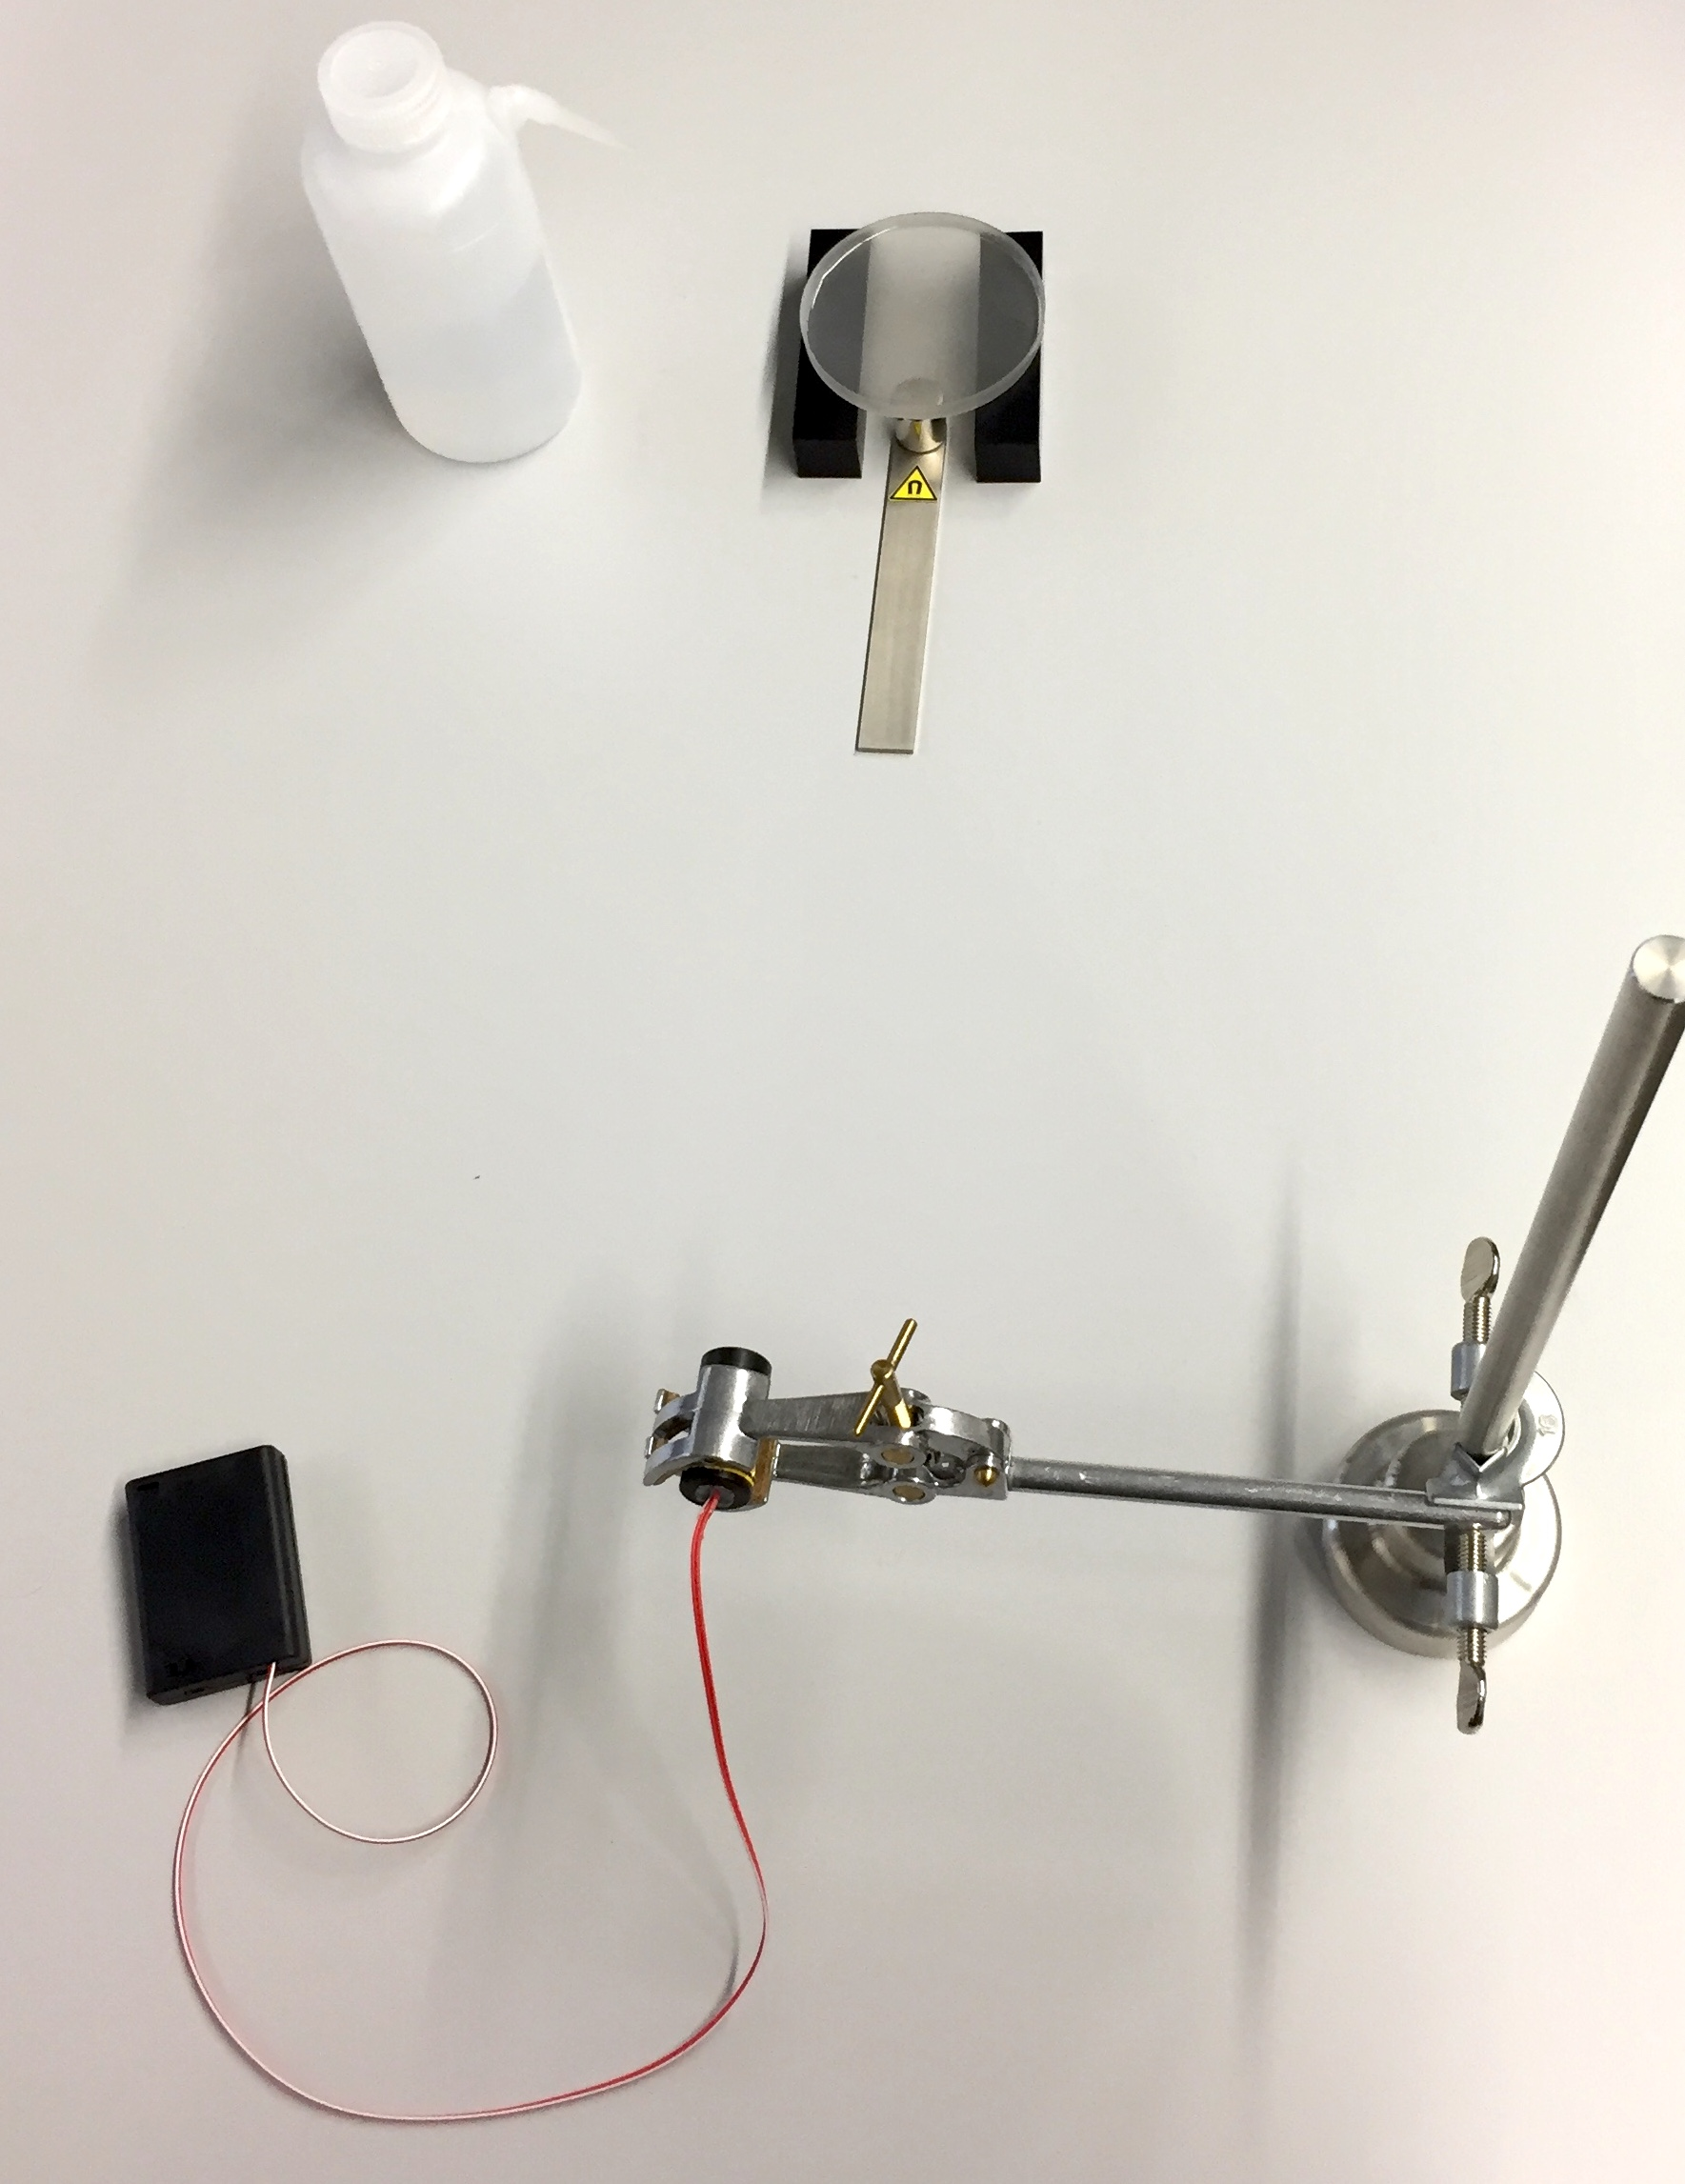
\includegraphics[width=0.5\textwidth]{res/Wasser.jpg}
	\caption{Zusehen ist hier der Versuchsaufbau mit dem der Einfluss eines Magnetfeldes auf Wasser untersucht wurde\protect\footnotemark.}
	\label{fig:Aufbau}
\end{figure}
\footnotetext{Entnommen am 20.11.17  aus dem Learnweb Kurs "Experimentelle Übungen I 17-18"}
\section{Einfluss eines Magneten auf eine Aluminiumplatte und auf einen Aluminiumkamm }\label{kap:Kamm_Platte}
Bei diesem Experiment ging es darum das verhalten zweier unterschiedlich geformter Körper aus dem gleichem Material zu untersuchen. Der Versuchsaufbau ist in \cref{fig:Alukamm} zu sehen.
Um das verhalten der Platte und des Kammes zu untersuchen wurde eine Reihe aus drei Magneten einmal schnell auf die Platte zubewegt und wieder entfernt und danach langsam angenähert und langsam wieder entfernt. Diese Aktionen wurden danach bei dem Kamm wiederholt.
Beim schnellen annähern an die Platte schwang die Platte zurück und beim langsamen entfernen wurde sie mitgezogen.
Dieses verhalten ist auf Diamagnetismus beziehungsweise Paramagnetismus zurückzuführen. Beim schnellen annähern tritt der Diamagnetismus auf und die Platte wurde aus dem Magnetfeld verdrängt. Entfernt man die Magneten jedoch langsam wieder überlagern die deutlich stärkeren Paramagnetischen Effekte den Diamagnetismus und die Platte wird mitgezogen.
Das bei dem Kamm nur der Paramagnetismus auftritt und das auch nur sehr schwach ist auf die Unterbrechungen in der Oberfläche zurückzuführen. Diese Unterbrechungen sorgen dafür das die Wirbelströme die auf die Oberfläche induziert werden deutlich schwächer ausfallen als bei der Platte.
Dadurch wird der sowieso schon sehr schwache Diamagnetische Effekt so stark abgeschwächt das er bei einem so schwachen Magnetfeld nicht mehr zu sehen ist.
\begin{figure}[h]
	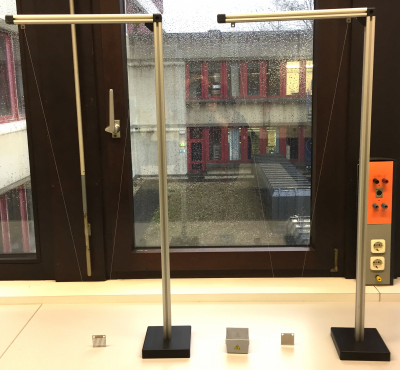
\includegraphics[width=0.5\textwidth]{res/Alupendel.png}
	\caption{In dieser Abbildung ist der Versuchsaufbau zu sehen mit dem man den Einfluss eines Magneten auf eine Aluplatte und auf einen Alukamm untersucht wurde\protect\footnotemark.}
	\label{fig:Alukamm}
\end{figure}
\footnotetext{Entnommen am 20.11.17  aus dem Learnweb Kurs "Experimentelle Übungen I 17-18"}

\section{Verhalten eines Magneten beim Fall durch ein Aluminiumrohr mit und ohne Schlitz.}

Dieses Experiment untersucht das gleiche verhalten das auch schon in \cref{kap:Kamm_Platte} zu beobachten war.
Hier wurde ein Magnet erst durch ein Rohr ohne Unterbrechungen in der Mantelfläche fallen gelassen und danach durch ein Rohr das an der Seite einen Schlitz hatte sodass die Oberfläche vollständig unterbrochen war (vgl. \cref{fig:Rohr}).
Beobachtet wurde bei der Durchführung das der Magnet durch das nicht ganz geschlossene Rohr zwar Langsamer fällt als wenn man ihn einfach so fallen gelassen hätte. Jedoch deutlich schneller als durch das Rohr mit dem nicht durchbrochenem Mantel. Dies ist eben genau auf diese Unterbrechung zurückzuführen, denn diese verhindert das schon in\cref{kap:Kamm_Platte} angesprochene induzieren von Wirbelströmen auf die Oberfläche des Rohrs. Da dies verhindert wurde ist der auftretende Paramagnetische Effekt ungleich kleiner als bei der Vollständig geschlossenen Röhre wo dies möglich ist. 
\begin{figure}[h]
	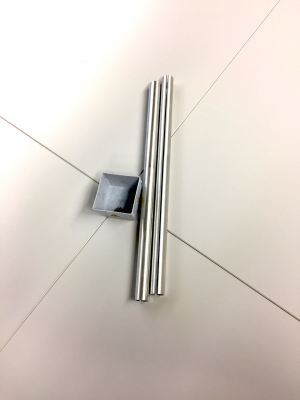
\includegraphics[width=0.5\textwidth]{res/Rohr.png}
	\caption{In dieser Abbildung sind die in diesem Experiment verwendeten Aluminiumrohre zu sehen\protect\footnotemark.}
	\label{fig:Rohr}
\end{figure}
\footnotetext{Entnommen am 20.11.17  aus dem Learnweb Kurs "Experimentelle Übungen I 17-18"}
\input{tex/15_Volumensuszebilität.tex}
%16
\section{Schlussfolgerung}




% --- Anhang einbinden
\IfFileExists{tex/20_Anhang.tex}{
	\clearpage
	\appendix
	\section{Anhang}
	\label{sec:anhang}
	

\subsection{Verwendete Gleichungen}\label{VGuD}
%und Definition der Variablen


%Zusammenhang zwischen Kreisfrequenz $\omega$ und Schwingungsdauer $T$:

%\begin{align}
%	T=\frac{2 \pi}{\omega} \pm \Delta t
%	\label{eq:T}
%\end{align} 


%Alle anderen Unsicherheiten sind gemäß Kapitel \ref{sec:einzeln} so klein, dass sie zu vernachlässigen sind. Es sei $\Delta t={ 0,006} {s}$.\\
%\frac{2 \pi}{\omega^2} \cdot\Delta \omega  \label{eq:T}


%Standardunsicherheit der Rechteckverteilung u für die Intervallbreite a:
	%\begin{align}
	%	u=\frac{a}{2\sqrt{3}}\label{eq:SR}
	%\end{align} 



}{}

% --- Literaturverzeichnis mit BibLaTeX
\ifthenelse{\boolean{showBibliography}}{
	\clearpage
	\printbibliography
}{}

\end{document}

